\section{Experimentos y resultados}
Cada experimento se hace con un script que guarda sus resultados en un CSV. Aquí vamos a leer los resultados y exponerlos, siguiendo el orden en el que los hemos ido haciendo. Dos utilidades que usamos en todas las secciones son: una función para el contraste por pares y otra para leer los datos de los CSV.

\subsection{CMA-ES sobre Diabetes y California}
El primer experimento es el del notebook prncipal de la práctica. Aprendimos $\theta$ con CMA-ES --- fitness : media de regresión lineal y KNN con 2020 evaluaciones --- en 13 particiones de cada uno de los dos datasets. Aquí recalculamos los errores de lso datos originales --- los \textit{e} del enunciado --- y los comparamos con los de CMA-ES. Estos resultados los recogemos en la \autoref{tab:resultados-finales}

\begin{table}[h]
\centering
\begin{tabular}{llrrrcr}
\hline
\textbf{Dataset} & \textbf{Modelo} & $\boldsymbol{e}$ & $\boldsymbol{e'}$ & \textbf{Cambio} & \textbf{Mejora en} & $\boldsymbol{p}$ \textbf{(Wilcoxon)} \\
\hline
california & KNN               & $0.826$  & $0.299$  & $-63.8$\,\% & 13/13 & $0.0002$ \\
           & Regresión lineal  & $0.533$  & $0.486$  & $-8.7$\,\%  & 13/13 & $0.0002$ \\
           & Árbol de decisión & $0.463$  & $0.462$  & $-0.2$\,\%  & 11/13 & $0.0134$ \\
\hline
diabetes   & KNN               & $47.100$ & $48.183$ & $+2.5$\,\%  & 4/13  & $0.1677$ \\
           & Regresión lineal  & $44.904$ & $45.011$ & $+0.2$\,\%  & 4/13  & $0.0681$ \\
           & Árbol de decisión & $61.948$ & $62.510$ & $+0.9$\,\%  & 7/13  & $0.8926$ \\
\hline
\end{tabular}
\caption{MAE con los atributos originales ($e$) y con la transformación aprendida ($e'$), promediado sobre 13 particiones. \emph{Mejora en} indica en cuántas particiones $e' < e$; $p$ es el p-valor del test de Wilcoxon de rangos con signo.}
\label{tab:resultados-finales}
\end{table}

La \autoref{fig:cambio-mae-particiones} nos muestra el cambio del MAE al aplicar la transformación aprendida. Cada punto es una partición, y la raya negra es la media. Los puntos por debajo de cero son mejoras. Lo que interesa mirar es la dispersión, y aque si todos los puntos están en el mismo lado del cero, la mejora es consistente. Si están repartidos en ambos lados, la media no significa nada.

En la \autoref{fig:cambio-mae-particiones} vemos que en California la mejora es sistemática. Los 13 puntos de KNN están apiñados en torno a un -64\%, y en regresión lineal todos caen alrededor de un 9\%. Por eso el valor de Wilcoxon es tan bajo. 

\begin{figure}[h]
\centering
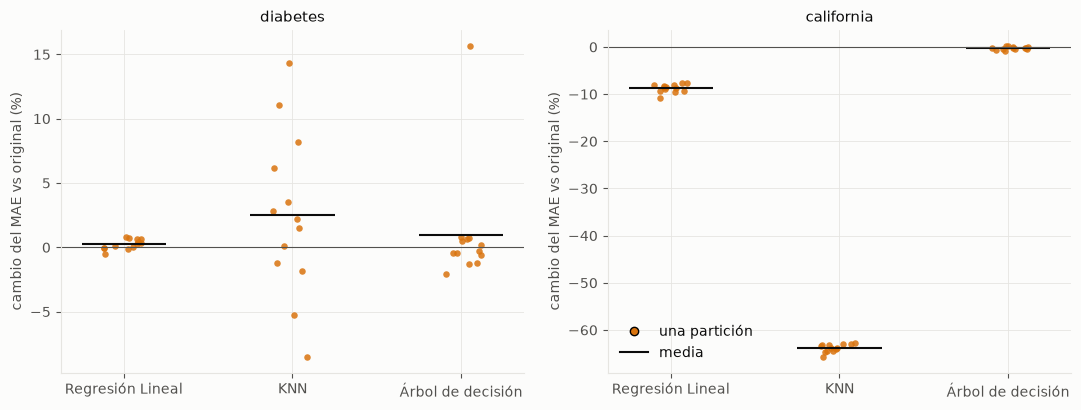
\includegraphics[width=\textwidth]{img/cambio_mae_particiones.png}
\caption{Cambio del MAE al aplicar la transformación aprendida, respecto a los atributos originales, en cada una de las 13 particiones. Cada punto es una partición y la línea negra, la media. Valores negativos indican mejora.}
\label{fig:cambio-mae-particiones}
\end{figure}

En Diabetes la media de KNN esconde una dispersión enorme que va desde un -8\% a un 14\%. Esto no necesariamente quiere decir que la transformación empeore de forma consistente, sino que es inestable para este dataset. Con tan pocos datos, la métrica aprendida acaba sobreajustándose en unas particiones, mientras que consigue acertar en otras. 

Pasando al árbol de decisión en Diabetes, hay un punto en 15\% que tira de la media hacia arriba, el resto se reparte en torno a cero. Es coherente con el valor de p=0.89, porque el test de rangos no se deja arrastrar por un valor extremo tanto como la media. En California el cambio es prácticamente nulo, lo cual tiene sentido dado que los árboles son invariantes a transformaciones monótonas por atributo; una métrica que reescala atributos apenas les afecta. 

Con estos resultados nos preguntamos si realmente importa el algorirmo evolutivo, qué ocurre en otros datasets y si se puede mejorar la representación o la regla de predicción. 

\subsection{Los datasets}
Antes de generalizar, tenemos que ver con qué clase de datos estamos trabajando. La \autoref{tab:datasets} muestra el número de muestras y de atributos de cada dataset (después de habernos quedado solo con los atributos numéricos y de limitar a 10.000 filas).

\begin{table}[h]
\centering
\begin{tabular}{lrrl}
\hline
\textbf{Dataset} & \textbf{Muestras} & \textbf{Atributos} & \textbf{Origen} \\
\hline
diabetes                                 & 442        & 10 & práctica \\
california                               & 20\,640    & 8  & práctica \\
\hline
concrete\_compressive\_strength          & 1\,030     & 8  & OpenML \\
stock                                    & 950        & 9  & OpenML \\
space\_ga                                & 3\,107     & 6  & OpenML \\
sulfur                                   & 10\,000    & 6  & OpenML \\
kin8nm                                   & 8\,192     & 8  & OpenML \\
bank8FM                                  & 8\,192     & 8  & OpenML \\
puma8NH                                  & 8\,192     & 8  & OpenML \\
house\_8L                                & 10\,000    & 8  & OpenML \\
cpu\_small                               & 8\,192     & 12 & OpenML \\
wine\_quality                            & 6\,497     & 11 & OpenML \\
\hline
\end{tabular}
\caption{Conjuntos de datos utilizados: los dos de la práctica y diez de regresión adicionales de OpenML.}
\label{tab:datasets}
\end{table}

Como se puede observar, son datasets pequeños o medianos, con entre 6 y 12 atributos numéricos. Los hemos escogido principalmente porque estaban diseñados para tareas de regresión, por su tamaño manejable y por su disponibilidad en OpenML. 

\subsection{Comparación con otras técnicas bioinspiradas e importancia del algoritmo evolutivo.}

En el paper de referencia se clasifican los algoritmos evolutivos en cuatro familias: enjambres, bioinspirados no basados en enjambre, físicos y químicos. Quisimos averiguar si había otra técnica mejor que CMA-ES para este problema. 

\subsubsection{Diseño del test}
\begin{itemize}
    \item Los mismo 20 y 16 parámetros ($\theta$), el mismo fitness (media de regresión lineal y KNN como en el notebook principal) y el mismo presupuesto de 1.000 evaluaciones para todos. 
    \item 20 algoritmos, casi todos de la primera tabla del paper, usando la librería \texttt{mealpy}, un algoritmo genético propio, CMA-ES, una búsqueda aleatoria y el punto inicial sin búsqueda. 
    \item El punto inicial $\theta_0$ se incluye en la población de partida de todos para que ninguno parta con desventaja. 
    \item Dos particiones por dataset - test rápido de carácter exploratorio.
\end{itemize}

Hay que tener cuidado porque algoritmos como BFO, CSO, CSA y FFA gastan muchas evaluaciones por iteración. Con 1000 evaluaciones, apenas consiguen completar una generación, por lo que sus resultados son básicamente los de elegir el mejor de unos 30 puntos aleatorios. No sacaremos conclusiones sobre ellos. En la \autoref{tab:rango-algoritmos} podemos ver el rango medio de cada algoritmo según el fitness alcanzado. 

\begin{table}[h]
\centering
\begin{tabular}{lr}
\hline
\textbf{Algoritmo} & \textbf{Rango medio} \\
\hline
CMA-ES             & $2.0$ \\
GA (propio)        & $2.5$ \\
BBO (biogeografía) & $3.5$ \\
HS (armonía)       & $3.5$ \\
DE                 & $4.5$ \\
ICA (imperialista) & $6.5$ \\
ACOR               & $7.5$ \\
ABC                & $7.5$ \\
\hline
\end{tabular}
\caption{Rango medio de cada algoritmo según el fitness alcanzado (1 = mejor).}
\label{tab:rango-algoritmos}
\end{table}

En la \autoref{fig:comparativa-algoritmos}, la barra es la media del cambio del MAE de validación (promedio de regresión lineal y KNN) en las dos particiones. Las barras hacia la izquierda se pueden interpretar como mejoras. Lo que hay que comparar, no obstante, es la diferencia entre los algoritmos, y hay que mirarla en relación a la que hay entre el punto inicial sin búsqueda, y la búsquea aleatoria (barras azules), que es lo que se consigue ''sin esfuerzo''. 

\begin{figure}[h]
\centering
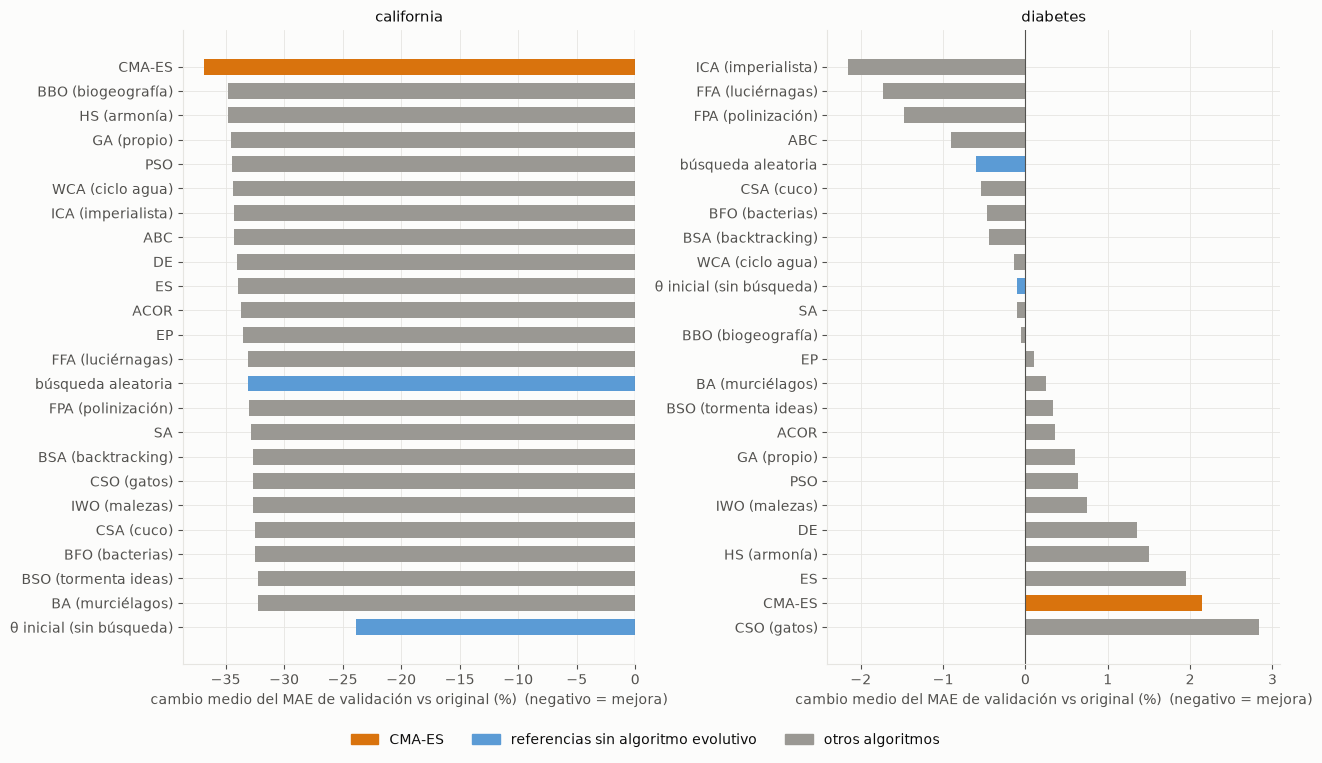
\includegraphics[width=\textwidth]{img/comparativa_algoritmos.png}
\caption{Cambio medio del MAE de validación respecto a los atributos originales para cada algoritmo de optimización. En naranja, CMA-ES; en azul, las referencias sin algoritmo evolutivo (parámetros iniciales y búsqueda aleatoria). Valores negativos indican mejora.}
\label{fig:comparativa-algoritmos}
\end{figure}

Podemos ver que en California casi todos los algoritmos consiguen entre un 32\% y un 37\% de mejora. Incluso la búsqueda aleatoria logra un 33\%. CMA-ES es el primero por poco, siendo la distancia entre los mejores algoritmos de 2-3 puntos con solo dos particiones. Por ello esto debe cogerse por pinzas y no es concluyente. Lo que importa es la familia de transformaciones, no el algoritmo que la busca.

En Diabetes ningún algoritmo mejora de forma fiable, las barras van de -2\% a 3\% y además tienen mucho ruido. CMA-ES sigue tenienod el mejor fitness, pero en validación empeora KNN. El cuello de botella, por ende, no es la potencia de búsqueda. 

Nos quedamos con CMA-ES porque tiene el mejor rango medio por fitness (2.0 seguido de cerca por el GA propio con 2.5). Es de los más baratos en tiempo y está justificado teóricamente para este tipo de porblemas continuo, sin gradiente y no separable. No es la única opción razonable, pero es la que se ha escogido. 

\subsection{¿Se puede mejorar CMA-ES con un híbrido?}
Como Diabetes fallaba por sobreajuste al fitness, probamos a diseñar un algoritmo nuevo que mezclara lo mejor de varios, partiendo del CMA-ES y probando cuatro modificaciones, cada una pensada para un problema concreto. Estas modificaciones quedan descritas en la \autoref{tab:variantes-hibridas} Además todas se evalúan con 1.000 evaluaciones y 5 particiones por dataset. 

\begin{table}[h]
\centering
\begin{tabular}{p{2.6cm}p{6.8cm}p{3.6cm}}
\hline
\textbf{Variante} & \textbf{Qué añade} & \textbf{Para qué} \\
\hline
CMA+folds & Cambia los pliegues de validación cruzada en cada generación (el fitness pasa a ser estocástico) & Que la búsqueda no se ajuste a unos pliegues concretos \\
\hline
CMA+DE & Inyecta en cada generación un individuo de cruce diferencial (de evolución diferencial) & Más diversidad, algo propio de DE y los algoritmos genéticos \\
\hline
CMA+folds+sel & Lo primero más una selección final: reservamos 100 evaluaciones para puntuar los mejores candidatos en pliegues nuevos, y solo aceptamos el aprendido si mejora a $\theta_0$ en más de $0.005$ & Elegir de forma robusta \\
\hline
Híbrido completo & Pliegues cambiantes, DE y selección final & Todo junto \\
\hline
\end{tabular}
\caption{Variantes híbridas de CMA-ES evaluadas.}
\label{tab:variantes-hibridas}
\end{table}

En la \autoref{tab:resultados-hibridos} podemos ver la diferenci amedia del cambio del MAE (puntos porcentuales) entre cada una de las variantes respecto al CMA-ES base, sobre 6 particiones. Valores positivos nos indican que la variante ha empeorado sus resultados. La columna ''Mejor que base'' cuenta cuántas de las particiones han conseguido mejorar a CMA-ES. 

\begin{table}[h]
\centering
\begin{tabular}{llrcr}
\hline
\textbf{Dataset} & \textbf{Variante} & \textbf{Dif. media (p.p.)} & \textbf{Mejor que base} & $\boldsymbol{p}$ \textbf{(Wilcoxon)} \\
\hline
california & CMA+folds              & $+7.09$ & 0/6 & $0.031$ \\
           & CMA+DE                 & $-0.28$ & 4/6 & $0.562$ \\
           & CMA+folds+sel          & $+0.40$ & 3/6 & $0.562$ \\
           & Híbrido (folds+DE+sel) & $+0.30$ & 2/6 & $0.688$ \\
\hline
diabetes   & CMA+folds              & $+1.24$ & 3/6 & $0.688$ \\
           & CMA+DE                 & $+1.53$ & 3/6 & $0.438$ \\
           & CMA+folds+sel          & $+0.98$ & 1/6 & $0.312$ \\
           & Híbrido (folds+DE+sel) & $+1.57$ & 0/6 & $0.031$ \\
\hline
\end{tabular}
\caption{Diferencia media, en puntos porcentuales de cambio del MAE, entre cada variante y CMA-ES base, sobre 6 particiones. Valores positivos indican que la variante es peor. \emph{Mejor que base} cuenta las particiones en que la variante mejora a CMA-ES.}
\label{tab:resultados-hibridos}
\end{table}

Adicionalmente, la \autoref{fig:variantes-hibridas} nos muestra de manera visual este cambio medio del MAE. Las barras representan la media en 6 particiones, mientras que la línea vertical sobre ellas representa la desviación típica entre las particiones. Si las líneas de dos variantes se solapan demasiado, la diferencia entre ellas pasa a no ser fiable. 

\begin{figure}[h]
\centering
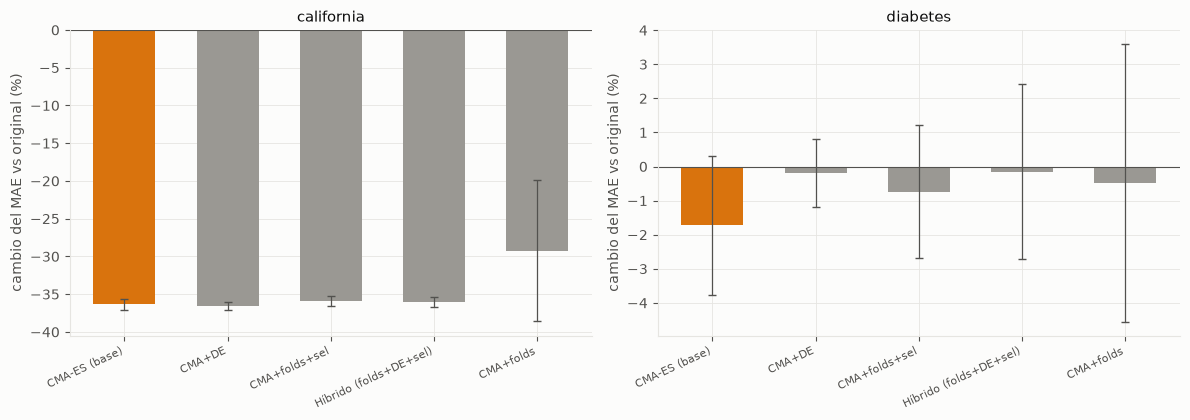
\includegraphics[width=0.8\textwidth]{img/variantes_hibridas.png}
\caption{Cambio medio del MAE respecto a los atributos originales para CMA-ES base (en naranja) y sus variantes híbridas, sobre 6 particiones. Las barras de error indican la desviación típica entre particiones. Valores negativos indican mejora.}
\label{fig:variantes-hibridas}
\end{figure}

Vemos que ninguna variante mejora al CMA-ES base. En California, DE y la selección robusta no cambian nada: tenemos diferencias de décimas de punto. En Diabetes ninguna mejora y el híbrido completo es peor en las seis particiones. Además, los pliegues cambiantes empeoran de manera clara en California. Unos siete puntos porcentuales peor, con una dispersión entre las particiones casi trece veces mayor. Esto puede deberse a que en cada generación se están comparando a candidatos con un ruido distinto y CMA-ES --- que se apoya en ordenar bien a los candidatos de una generación --- avanza peor. Nuestra hipótesis era que este híbrido conseguiría reducir el sobreajuste en Diabetes, pero no hemos podido confirmarlo. 

Lo que aprendemos de esta sección es que inventar un algoritmo nuevo no tenía sentido en este punto. Lo que mueve los resultados son la representación y la regla de predicción, no la búsqueda en sí. Por ello, el resto de experimentos los centraremos en esto. 

\subsection{Introducción de PCA dentro de la búsqueda para la reducción de ruido. }

La idea es que la propia búsqueda decida qué componentes principales conservar, como un método alternativo de reducir el ruido. La representación pasaría a ser: 
\begin{enumerate}
    \item Yeo-Johnson 
    \item Estandarización 
    \item Pesos por atributo 
    \item PCA
    \item Pesos por componente
\end{enumerate}

Con todos los pesos en 1 es una rotación, y las distancias son idénticas a las de la estandarización,  por lo que la búsqueda también arranca de la línea base. El peso de cada componente lo aprende CMA-ES: un peso cercano a 0 equivale a descartar ese componente (reducción de ruido aprendido). Añade $n$ parámetros ($3n$ en total). Probamos también una variante con solo dos parámetros --- un corte y una suavidad --- y la comparamos con el PCA clásico que conserva el 95\% de la varianza.

El diseño lo hacemos en dos fases para evitar el sesgo de selección. Una primera tanda con semillas del 13 al 15 se usan para elegir la variante, y una tanda de confirmación con 10 particiones nuevas (semillas de 30 a 39) que permite decidir antes de mirar que el PCA solo entraría en el método final si mejoraba de forma consistente. Las siguientes gráficas usan la tanda de confirmación. En la \autoref{tab:comparativa-pca} vemos que la versión con PCA mejora solo en un 0.003, una diferencia no significativa. Esto nos puede indicar que una rotación de los ejes no aporta nada sobre reescalar los atributos originales.

\begin{table}[h]
\centering
\begin{tabular}{lr}
\hline
\textbf{Transformación} & \textbf{KNN} \\
\hline
Crudo                              & $1.000$ \\
Estándar                           & $0.871$ \\
CMA-ES (YJ + pesos)                & $0.748$ \\
CMA-ES + PCA (peso por componente) & $0.745$ \\
\hline
\end{tabular}
\caption{MAE de KNN con cada transformación, relativo al obtenido con los atributos originales (crudo = 1).}
\label{tab:comparativa-pca}
\end{table}

\begin{figure}[h]
\centering
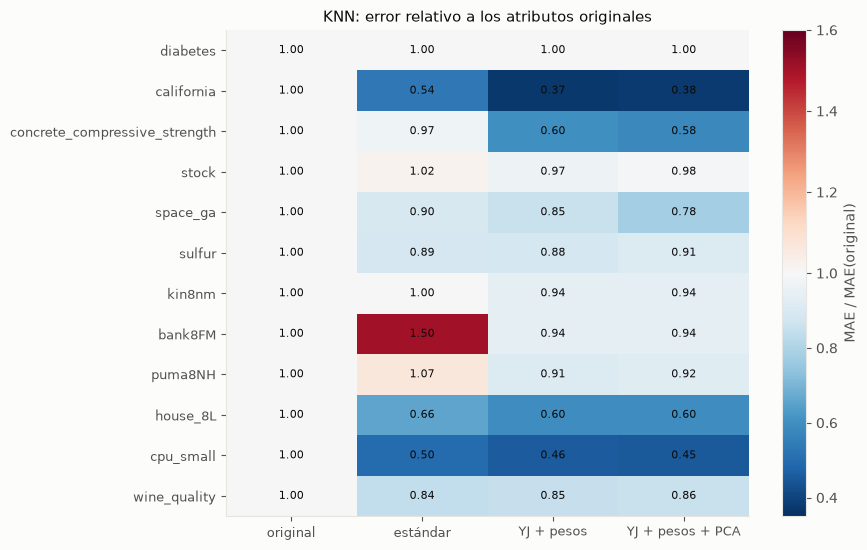
\includegraphics[width=0.85\textwidth]{img/heatmap_knn_datasets.png}
\caption{MAE de KNN con cada transformación, relativo al obtenido con los atributos originales, en los 12 datasets. Azul indica mejora (valor menor que 1) y rojo, empeoramiento.}
\label{fig:heatmap-knn}
\end{figure}

En la \autoref{fig:heatmap-knn} vemos un mapa de calor donde cada celda es el cociente entre el error de ese método y el del dataset con los atributos originales. Los valores son, por ende, la media geométrica de las columnas. Por debajo de 1 (azul) se mejora, y por encima del 1 (naranja) empeora. Una columna de azules uniformes nos indica que el método funciona por lo general, mientras que una fila de naranjas indica un dataset difícil. 

Se observa que estandarizar solo mejora en unos datasets y empeora en otros --- por ejemplo el de banca, donde ya parte de un putno mucho peor que los datos originales. La columna de ''YJ + pesos'' es mucho más azul que ''estándar'', mejorando en 11/12 datasets. Además, concluimos que añadir el PCA apenas cambia la columna, ya que se ve casi igual que la de ''YJ + pesos''. De hecho, en la \autoref{fig:efecto-pca} podemos ver el cambio medio del error al añadir PCA por dataset (barras). Un asterisco indica que ese cambio es estadísticamente distinguible de cero con 10 particiones. Si las barras se reparten a ambos lados, el efecto medio se anula; y esto es lo que observamos en la mayoría de casos.

\begin{figure}[h]
\centering
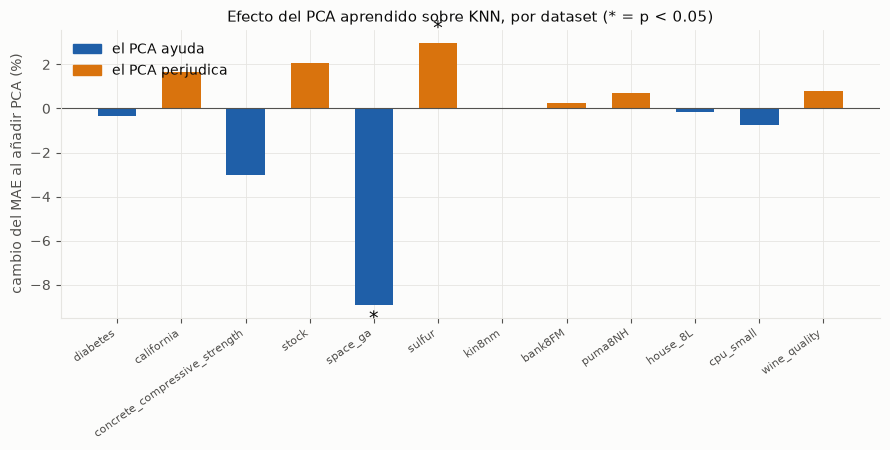
\includegraphics[width=0.75\textwidth]{img/efecto_pca_knn.png}
\caption{Cambio del MAE de KNN al añadir la rotación PCA a la transformación aprendida (YJ + pesos), por dataset. En azul, los datasets donde PCA mejora; en naranja, donde empeora. El asterisco marca diferencias significativas ($p < 0.05$, test de Wilcoxon).}
\label{fig:efecto-pca}
\end{figure}

Se observa que en conjunto, el PCA apenas aporta nada. El cambio global es de apenas un -0.4\% y el p-valor se acerca a 1. Con el criterio fijado, el PCA queda por fuera del método final. Aunque eso no quiere decir que no ayude en todos los datasets, de hecho, aporta bastante en \texttt{space\_ga} (alrededor de un 9\% menos de error, mejorando en todas las particiones). Esto puede deberse a que los atributos ya estaban de partida muy correlacionados, que es donde rotar puede tener sentido. Sin embargo, perjudica a otros datasets como \texttt{sulfur} y \texttt{stock}. 

El PCA clásico con el corte en el 95\% de varianza empeora la estandarización en la primera tanda --- 0.896 frente a 0.873 de media --- por lo que quitar componentes de forma fija no parece ser la mejor forma de reducir el ruido. 

En la primera tanda de 3 particiones el PCA parecía mejorar en los 12 datasets, pero cuando lo intentamos confirmar con más particiones nuevas la ventaja despaarece. Por eso insistimos en usar particiones que no se usaron para elegir a la hora de evaluar si los cambios en el método son significativos. 

\subsection{Cambiar la regla de predicción: regresión lineal local.}
Como lo que mueve los resultados es la regla de predicción y no el algoritmo evolutivo, vamos a probar con una regla local lineal. El experimento separa dos preguntas con cinco configuraciones: 6 particiones nuevas en cada uno de los 12 datasets. Estas preguntas y configuraciones se recogen en la \autoref{tab:comparaciones}.

\begin{table}[h]
\centering
\begin{tabular}{p{5.5cm}p{7.5cm}}
\hline
\textbf{Configuración} & \textbf{Qué responde} \\
\hline
estándar + KNN y estándar + LLR & ¿Ayuda la regla por sí sola, sin aprender nada? \\
\hline
métrica(KNN) + KNN y métrica(KNN) + LLR & Con la misma métrica, ¿ayuda cambiar la regla? \\
\hline
métrica(LLR) + LLR & ¿Ayuda optimizar la métrica directamente para la regla? \\
\hline
\end{tabular}
\caption{Comparaciones planteadas entre configuraciones y la pregunta que responde cada una.}
\label{tab:comparaciones}
\end{table}

En las cuatro primeras $k$ y el ridge se eligen por validación cruzada en una rejilla de 15 combinaciones. En la última los aprende CMA-ES junto con la métrica. Esa última configuración es el método completo. 

En la \autoref{tab:resultados-llr} podemos ver el MAE de cada configuración en relación al de KNN con los atributos originales. Con esto podemos responder a las tres preguntas de la tabla anterior. En primer lugar, que la regla de por sí ayuda, ya que el paso de KNN a LLR con atributos estandarizados --- 0.840 a 0.737 --- da casi lo mismo que aprender la métrica para KNN (0.724) sin optimizar nada. Además, con la misma métrica, vemos que cambiar la regla ayuda, pasando de un 0.724 a un 0.673 en meida (geométrica). Finalmente, también comprobamos que ayuda optimizar la métrica para la regla, aunque la ganancia es más pequeña.

\begin{table}[h]
\centering
\begin{tabular}{lr}
\hline
\textbf{Configuración} & \textbf{MAE relativo} \\
\hline
estándar + KNN      & $0.840$ \\
estándar + LLR      & $0.737$ \\
métrica(KNN) + KNN  & $0.724$ \\
métrica(KNN) + LLR  & $0.673$ \\
métrica(LLR) + LLR  & $\mathbf{0.641}$ \\
\hline
\end{tabular}
\caption{MAE de cada configuración relativo al de KNN con los atributos originales (media geométrica sobre los 12 datasets). Menor es mejor.}
\label{tab:resultados-llr}
\end{table}

En la \autoref{fig:resultados-llr}, la gráfica de la izquierda muestra la media geométrica del cociente entre el error de cada método y el de KNN con los atributos originales (a menor valor, mejor). El mapa de color de la derecha desglosa dicho cociente por dataset. En la \autoref{tab:contrastes-llr}, \emph{Cambio} es la variación media del error entre los dos métodos que se comparan; \emph{Mejor en} cuenta en cuántos de los 72 casos gana el primero, y $p$ es el p-valor del test de Wilcoxon por pares.

\begin{figure}[h]
\centering
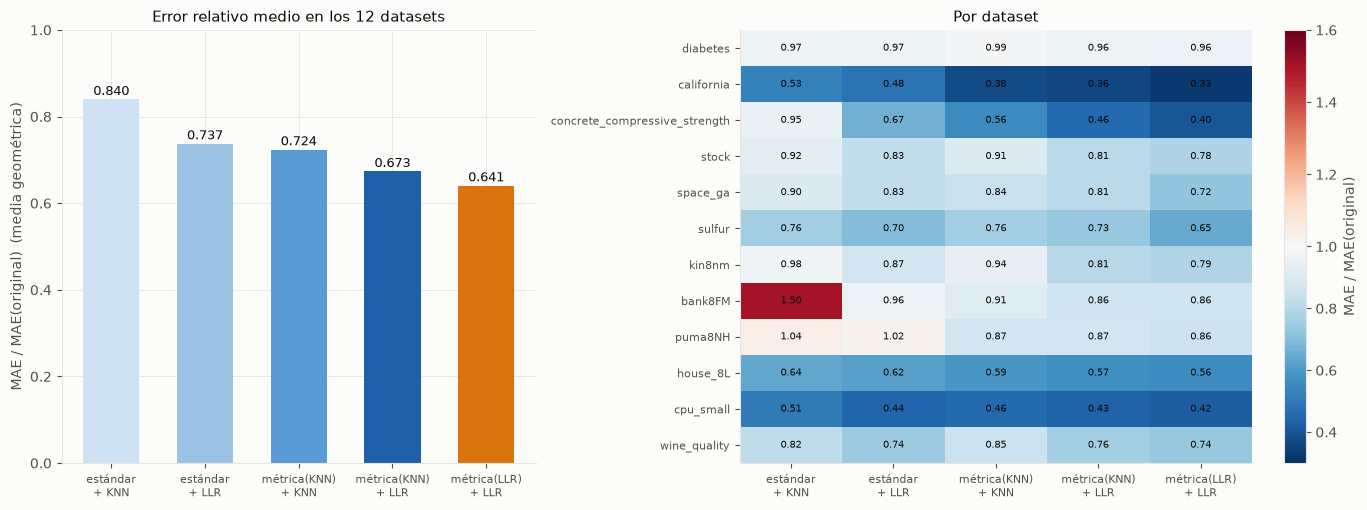
\includegraphics[width=\textwidth]{img/resultados_llr.png}
\caption{Izquierda: MAE relativo a KNN con los atributos originales, como media geométrica sobre los 12 datasets; en naranja, el método completo. Derecha: el mismo cociente por dataset. Azul indica mejora (valor menor que 1) y rojo, empeoramiento.}
\label{fig:resultados-llr}
\end{figure}

Vemos que cada paso mejora al anterior, la media geométrica baja de 0.84 (estándar + KNN) a 0.64 (método completo). Frente a los datos originales, obtenemos un 36\% menos de error. Además, vemos también que la regla local lineal ayuda por sí sola, ya que con datos estándar baja el error un 12\% respecto a KNN, ganando en 68 de 72 parejas. Una parte de la mejora del método completo viene de usar una regla más flexible, y no tanto de la métrica. Frente a la regla local sin aprender, el método completo baja el error un 13\%, y optimizar la métrica para la regla gana casi un 5\% a reutilizar la métrica de KNN con la regla local lineal. Es un cambio pequeño, pero consistente, ganando en 56 de 72 parejas. 

Adicionalmente, es consistente entre datasets. El método completo está por debajo de 1 en los 12 datasets. Las mayores mejoras llegan la 60-67\% de reducción del error, siendo el menor \texttt{diabetes}, donde solo llega a un 4\%. 

Algunas cosas a tener en cuenta son: primero, que la última configuración aprende \textit{k} y el ridge con 1000 evaluaciones de CMA-ES, mientras que las demás los eligen en una rejilla de 15 combinaciones. Parte de la ventaja puede ser simplemente más ajuste de hiperparámetros. Segundo, tarda mucho más.

\begin{table}[h]
\centering
\begin{tabular}{p{7cm}rcr}
\hline
\textbf{Comparación} & \textbf{Cambio} & \textbf{Mejor en} & $\boldsymbol{p}$ \textbf{(Wilcoxon)} \\
\hline
estándar + LLR frente a estándar + KNN \newline {\small (la regla sola)}                 & $-12.1$\,\% & 68/72 & $<0.0001$ \\
métrica(KNN) + LLR frente a métrica(KNN) + KNN \newline {\small (cambiar la regla)}       & $-6.9$\,\%  & 67/72 & $<0.0001$ \\
métrica(LLR) + LLR frente a métrica(KNN) + LLR \newline {\small (optimizar para la regla)} & $-4.9$\,\%  & 56/72 & $<0.0001$ \\
\hline
métrica(LLR) + LLR frente a estándar + LLR                                               & $-13.2$\,\% & 66/72 & $<0.0001$ \\
métrica(LLR) + LLR frente a estándar + KNN                                               & $-23.7$\,\% & 69/72 & $<0.0001$ \\
\hline
\end{tabular}
\caption{Contrastes entre configuraciones sobre 72 casos (12 datasets $\times$ 6 particiones). \emph{Cambio} es la variación media del MAE de la primera configuración respecto a la segunda; \emph{Mejor en} cuenta los casos en que la primera tiene menor error.}
\label{tab:contrastes-llr}
\end{table}

\subsection{¿Cómo queda frente a otros modelos a nivel absoluto?}
Que un método mejore a KNN no dice si es bueno en términos absolutos. Lo comparamos con los modelos que suelen ganar en datos tabulares: 

\begin{itemize}
    \item Random Forest con 200 árboles y Gradient Boosting (\texttt{HistGradientBoosting}) ajustados con una búsqueda aleatoria de 30 configuraciones y validación cruzada de 3 pliegues y reentrenados con todo el entrenamiento. 
    \item Proceso gaussiano con ARD --- una esclaa por atributo, estimada por máxima verosimilitud. Es el competidor teórico más cercano porque aprende justo lo que aprendemos nosotros, pesos por atributo. Lo entrenamos con una submuestra de 2000 filas por coste, lo que le da menos datos que a nuestro método. 
\end{itemize}

\begin{figure}[h]
\centering
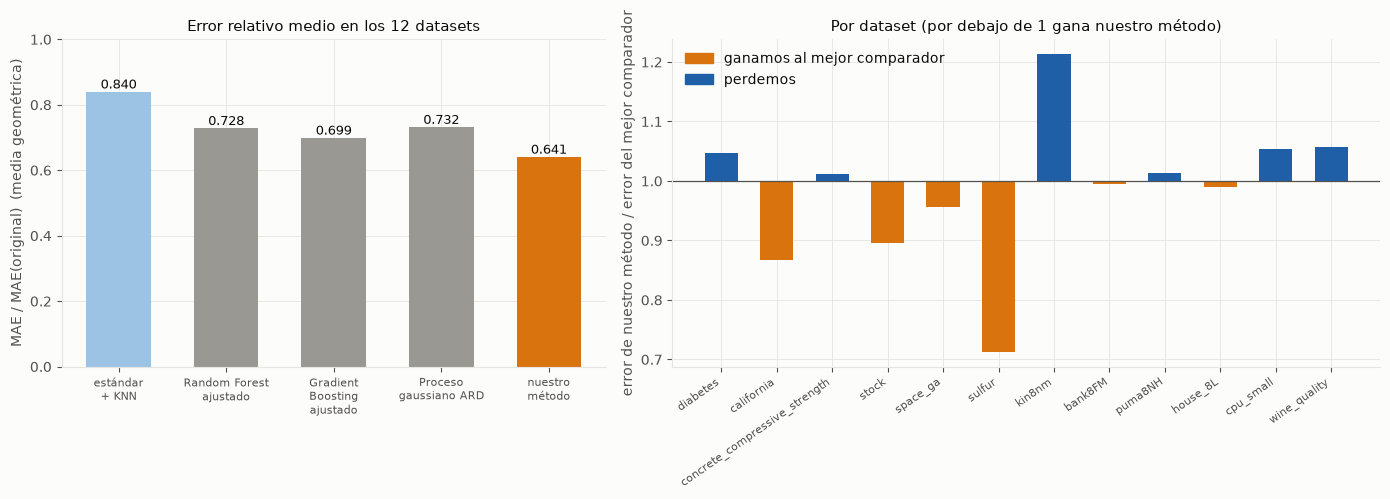
\includegraphics[width=\textwidth]{img/comparativa_modelos.png}
\caption{Izquierda: MAE relativo a KNN con los atributos originales (media geométrica sobre los 12 datasets) de nuestro método frente a otros modelos de regresión. Derecha: cociente entre el error de nuestro método y el del mejor de los comparadores en cada dataset; por debajo de 1, nuestro método gana.}
\label{fig:comparativa-modelos}
\end{figure}

En la \autoref{fig:comparativa-modelos}, a la izquierda nos fijamos en los errores relativos, a menor valor, mejor. Y a la derecha, cada barra representa el cociente entre el error de nuestro método y el del mejor de los tres comparadores del dataset: por debajo de 1 (naranja) ganamos, y por encima (azul), perdemos. Este cociente es una comparación dura, porque el mejor comparador se elige después de ver los resultados\dots

Vemos que de media nuestro método tiene el menor error, y frente a cada uno por separado la ventaja es del 8\% al 12\% y significativa (p de Wilcoxon). Además, frente al mejor de los tres en cada pareja, la diferencia es de aproximadamente un -2\%, lo cual en este caso no es significativo. Es decir, que estamos a la altura del mejor modelo de referencia, pero no por encima. Finalmente, por dataset hay ganadores distintos, por lo que el resultado también depende en gran medida de la naturaleza de los datos y atributos del problema.

\begin{table}[h]
\centering
\begin{tabular}{p{7cm}rcr}
\hline
\textbf{Comparación} & \textbf{Cambio} & \textbf{Mejor en} & $\boldsymbol{p}$ \textbf{(Wilcoxon)} \\
\hline
Nuestro método frente a Random Forest ajustado      & $-12.0$\,\% & 58/72 & $<0.0001$ \\
Nuestro método frente a Gradient Boosting ajustado  & $-8.3$\,\%  & 53/72 & $<0.0001$ \\
Nuestro método frente a proceso gaussiano ARD       & $-12.4$\,\% & 51/72 & $<0.0001$ \\
\hline
Nuestro método frente al mejor de los tres en cada dataset & $-2.1$\,\% & 33/72 & $0.618$ \\
\hline
\end{tabular}
\caption{Contrastes entre nuestro método y otros modelos de regresión sobre 72 casos (12 datasets $\times$ 6 particiones). \emph{Cambio} es la variación media del MAE de nuestro método respecto al comparador; \emph{Mejor en} cuenta los casos en que nuestro método tiene menor error.}
\label{tab:contrastes-modelos}
\end{table}

En la \autoref{tab:contrastes-modelos} podemos ver los contrastes entre nuestro modelo y los otros sobre los 72 casos. La última fila es la más interesante, ya que muestra que ganamos en menos de la mitad de los casos, pero con un cambio medio negativo de -2.1\%. Esto es interesante, porque cuando ganamso lo hacemos por más margen que cuando perdemos. No obstante, con un $p=0.618$ no hay diferencia significativa. Volvemos a la conclusión de que nuestro método está a la par del mejor modelo elegido a posteriori en cada dataset, y supera de forma significativa a cada uno de ellos por separado. 

Sin embargo, otro punto a tener en cuenta es que el proceso gaussiano solo ve 2000 filas, lo que perjudica en los datasets grandes. Nuestro método ajusta más hiperparámetros (exponentes, peso, k, ridge) que Random Forest y Gradient Boosting, que solo ajustan 30 configuraciones aleatorias. 

\subsection{Caso de Diabetes}
Diabetes es el único dataset de la práctica donde el método no cumple el criterio de $e' < e$, y necesitamos saber por qué. Mostramos el cambio del error por partición para los cuatro métodos de la confirmación en 10 particiones.

\begin{figure}[h]
\centering
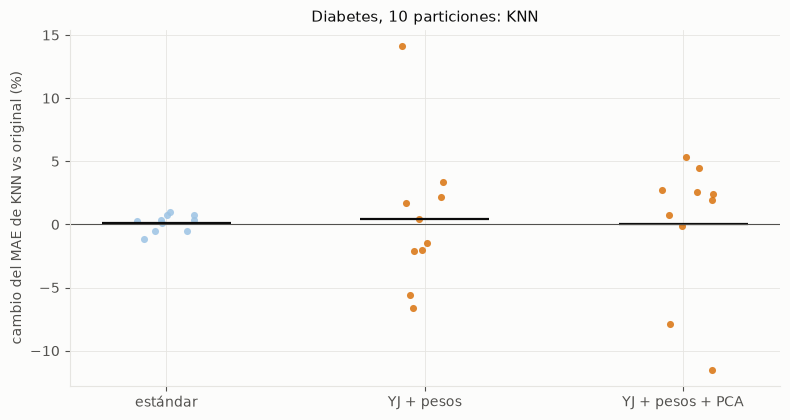
\includegraphics[width=0.7\textwidth]{img/diabetes_particiones_knn.png}
\caption{Cambio del MAE de KNN respecto a los atributos originales en diabetes, para cada una de las 10 particiones. Cada punto es una partición y la línea negra, la media.}
\label{fig:diabetes-particiones}
\end{figure}

\begin{table}[h]
\centering
\begin{tabular}{lrr}
\hline
\textbf{Transformación} & \textbf{Media} & \textbf{Desviación típica} \\
\hline
Estándar                                & $+0.13$\,\% & $0.66$ \\
CMA-ES (YJ + pesos)                     & $+0.40$\,\% & $5.80$ \\
CMA-ES + PCA (peso por componente)      & $+0.07$\,\% & $5.45$ \\
\hline
\end{tabular}
\caption{Media y desviación típica, sobre 10 particiones, del cambio del MAE de KNN respecto a los atributos originales en diabetes.}
\label{tab:diabetes-dispersion}
\end{table}

En la \autoref{fig:diabetes-particiones} vemos que los puntos están repartidos a ambos lados de cero, por lo que no podemos demostrar que haya una mejora. En la \autoref{tab:diabetes-dispersion} se recogen la media y la desviación típica sorbe las 10 particiones, respecto al cambio del MAE de KNN respecto a los atributos originales en diabetes. 

Con 10 particiones nuevas, el cambio medio es prácticamente nulo para todos los métodos, con una desviación de unos 5-6 puntos porcentuales entre particiones. Por ende, la conclusión es que no hay mejora en Diabetes. Esto se puede deber a la poca presencia de datos, con solo 309 muestras de entrenamiento para ajustar 20 parámetros con un fitness que usa validación cruzada sobre esas mismas muestras. La búsqueda mejora el fitness --- bajada de 5-8\% --- pero esa mejora no llega a trasladarse a validación: sobreajuste al criterio de búsqueda\dots

Probamos regularizar hacia $\theta_0$, usar un único exponente compartido, pliegues cambiantes y selección robusta con validación independiente; pero ninguna mejora Diabetes de forma consistente. Los propios datos explican que el margen sea bajo, ya que los datos ya vienen centralizados y escalas parecidas, por lo que estandarizar no cambia nada y tampoco hay colas largas que requieran de corrección. 

En una tanda con solo 2 particiones, CMA-ES sale con +2.2\% en Diabetes, y con 6 particiones con -1.7\% (en ambos casos, promedio de regresión lineal y KNN).El signo cambiaba con el número de particiones. Con una desviación de 5-6 puntos. Por ende, podemos concluir que cualquier interpretación sobre Diabetes con pocas particiones se basa en ruido.